\documentclass[11pt,a4paper]{ctexart}

\usepackage[margin=2.6cm]{geometry}
\usepackage{amsmath,amssymb,amsthm}
\usepackage{graphicx}
\usepackage{booktabs}
\usepackage{hyperref}
\usepackage{xcolor}
\usepackage{listings}
\usepackage{caption}

\graphicspath{{figures/}}
\hypersetup{colorlinks=true, linkcolor=blue!50!black, urlcolor=blue!60!black}
\lstset{
  basicstyle=\ttfamily\small,
  breaklines=true,
  frame=single,
  columns=fullflexible,
  backgroundcolor=\color{gray!7}
}

\newtheorem{definition}{定义}[section]
\newtheorem{theorem}{定理}[section]
\newtheorem{lemma}{引理}[section]
\newtheorem{proposition}{命题}[section]
\newtheorem{example}{例}[section]

\title{第 6 章 \quad Autocovariance and partial covariance / 自协方差与偏协方差}
\author{基于 \textit{A Course in Time Series Analysis} 的中文讲义与 Python 实践}
\date{}

\begin{document}
\maketitle

\section*{本章学习目标}

本章按照原文 \textit{The autocovariance and partial covariance of a stationary time series} 的小节顺序整理，保留主要定义、定理、模型公式和练习方向，并将原文中的 R 实践思路改写为 Python 工程实践。

完成本章后，应能够：
\begin{itemize}
  \item 推导线性过程、AR、MA、ARMA 的自协方差；
  \item 理解 ARMA 自协方差衰减速度；
  \item 估计样本 ACF 并识别模型；
  \item 定义时间序列偏协方差与 PACF；
  \item 理解方差矩阵、精度矩阵和非因果模型的 ACF。
\end{itemize}

\section{自协方差函数}

平稳过程的自协方差定义为
\[
  c(k)=\mathrm{cov}(X_t,X_{t+k}).
\]
对线性过程
\[
  X_t=\sum_{j=0}^{\infty}\psi_j\varepsilon_{t-j},
\]
若 \(\mathrm{var}(\varepsilon_t)=\sigma^2\)，则
\[
  c(k)=\sigma^2\sum_{j=0}^{\infty}\psi_j\psi_{j+|k|}.
\]

\begin{lemma}[线性表示的协方差，原文 Lemma 6.1.1]
若平稳序列具有绝对可和的线性表示，则其自协方差由系数卷积给出，并且 \(\sum_k|c(k)|<\infty\) 在相应条件下成立。
\end{lemma}

\subsection{ARMA 协方差的衰减}

因果可逆 ARMA 的系数通常几何衰减，因此自协方差也几何衰减。AR 根越接近单位圆，ACF 衰减越慢。

\section{AR、MA 和 ARMA 的自协方差}

AR(p) 模型
\[
  X_t=\phi_1X_{t-1}+\cdots+\phi_pX_{t-p}+\varepsilon_t
\]
两边同乘 \(X_{t-k}\) 并取期望，可得 Yule-Walker 方程：
\[
  c(k)=\phi_1c(k-1)+\cdots+\phi_pc(k-p),\qquad k\ge1.
\]
对 AR(1)，
\[
  c(k)=\frac{\sigma^2}{1-\phi^2}\phi^{|k|}.
\]

MA(q) 模型
\[
  X_t=\varepsilon_t+\theta_1\varepsilon_{t-1}+\cdots+\theta_q\varepsilon_{t-q}
\]
的自协方差在 \(q\) 阶后截尾：
\[
  c(k)=0,\qquad |k|>q.
\]
ARMA 模型的 ACF 通常在前若干阶受 MA 部分影响，随后按 AR 部分的差分方程递推衰减。

\section{从数据估计 ACF}

若均值未知，样本自协方差通常写为
\[
  \hat c(k)=\frac1n\sum_{t=1}^{n-k}(X_t-\bar X)(X_{t+k}-\bar X),
\]
样本自相关为
\[
  \hat\rho(k)=\frac{\hat c(k)}{\hat c(0)}.
\]
ACF 图是识别线性模型的基础：MA(q) 的 ACF 倾向截尾，AR(p) 的 ACF 倾向拖尾。

\section{偏相关}

\begin{definition}[偏协方差/偏相关，原文 Definition 6.2.1]
\(X_t\) 与 \(X_{t+h}\) 在控制中间变量 \(X_{t+1},\ldots,X_{t+h-1}\) 后的残差协方差称为偏协方差；标准化后称为偏相关。
\end{definition}

对平稳序列，h 阶偏自相关可记为 \(\phi_{h,h}\)。它等于用 \(X_{t-1},\ldots,X_{t-h}\) 预测 \(X_t\) 的最佳 AR(h) 模型中第 h 个系数。AR(p) 的 PACF 在 p 阶后截尾。

\section{方差矩阵、精度矩阵与非因果模型}

对向量 \(X_1,\ldots,X_n\)，协方差矩阵为 Toeplitz 形式：
\[
  \Gamma_n=(c(i-j))_{i,j=1}^n.
\]
其逆矩阵反映条件线性依赖结构。AR(p) 过程的精度矩阵具有带状结构，这对应“给定最近 p 个邻居后更远变量无直接线性影响”。

原文最后讨论非因果时间序列和 minimum phase。谱密度定义为
\[
  f(\omega)=\frac1{2\pi}\sum_{k=-\infty}^{\infty}c(k)e^{-ik\omega},
\]
不同因果/非因果表示可能具有相同的二阶结构，因此仅凭 ACF 不能总是区分时间方向。

\section{原文小节覆盖补充}

\subsection{ARMA 自协方差衰减速度}
因果 ARMA 的自协方差通常按几何速度衰减。AR 根越接近单位圆，衰减越慢；复根会导致振荡衰减。这解释了 ACF 图中拖尾和周期形态。

\subsection{AR 自协方差与 Yule-Walker 方程}
AR(p) 自协方差满足 Yule-Walker 递推。Exercise 6.1 和 Exercise 6.2 延续第 4 章 AR(2) 练习，要求推出 ACF 形状和周期。

\begin{example}[原文 \(p=2\) 例子]
若 \(\phi(z)=1-\phi_1z-\phi_2z^2\) 的根为复共轭，则 \(c(k)\) 是指数衰减和三角函数振荡的乘积。
\end{example}

\subsection{MA、ARMA 和样本 ACF}
MA(q) 的自协方差在 q 阶后截尾；ARMA(p,q) 在前 q 阶受 MA 部分影响，随后满足 AR 递推。样本 ACF 用 \(\hat c(k)/\hat c(0)\) 估计，但大滞后处不稳定。

\subsection{偏相关与 PACF 图}
偏协方差是去除中间变量线性影响后的残差协方差。h 阶 PACF 等于最佳 AR(h) 预测中最后一个系数。Exercise 6.3 研究可逆 MA(1) 的偏相关；Exercise 6.4 和 Exercise 6.5 比较 AR 与实际温度数据的 ACF/PACF。

\subsection{方差矩阵和非因果过程}
原文第 6.3 节研究 Toeplitz 方差矩阵和精度矩阵。第 6.4 节定义谱密度与 minimum phase，并讨论非因果 ARMA 的 Yule-Walker 方程和滤波。Exercise 6.6、Exercise 6.7、Exercise 6.8 分别对应 AR(2) 方差矩阵、精度矩阵性质和非因果 AR(p)。

\begin{definition}[minimum phase，原文 Definition 6.4.2]
若 ARMA 表示中 AR 和 MA 多项式的根都在单位圆外，则称该表示为 minimum phase；它对应因果且可逆的规范表示。
\end{definition}

\section{Python 工程实践}

在本章目录下运行：
\begin{lstlisting}[language=bash]
python scripts/ch06_generate_figures.py
\end{lstlisting}

脚本会把图像写入本章 \texttt{figures/} 目录。当前图像用于配合本章核心概念的仿真说明；若后续补齐原始数据文件，可把模拟数据替换为原文真实数据案例。

\begin{figure}[htbp]
  \centering
  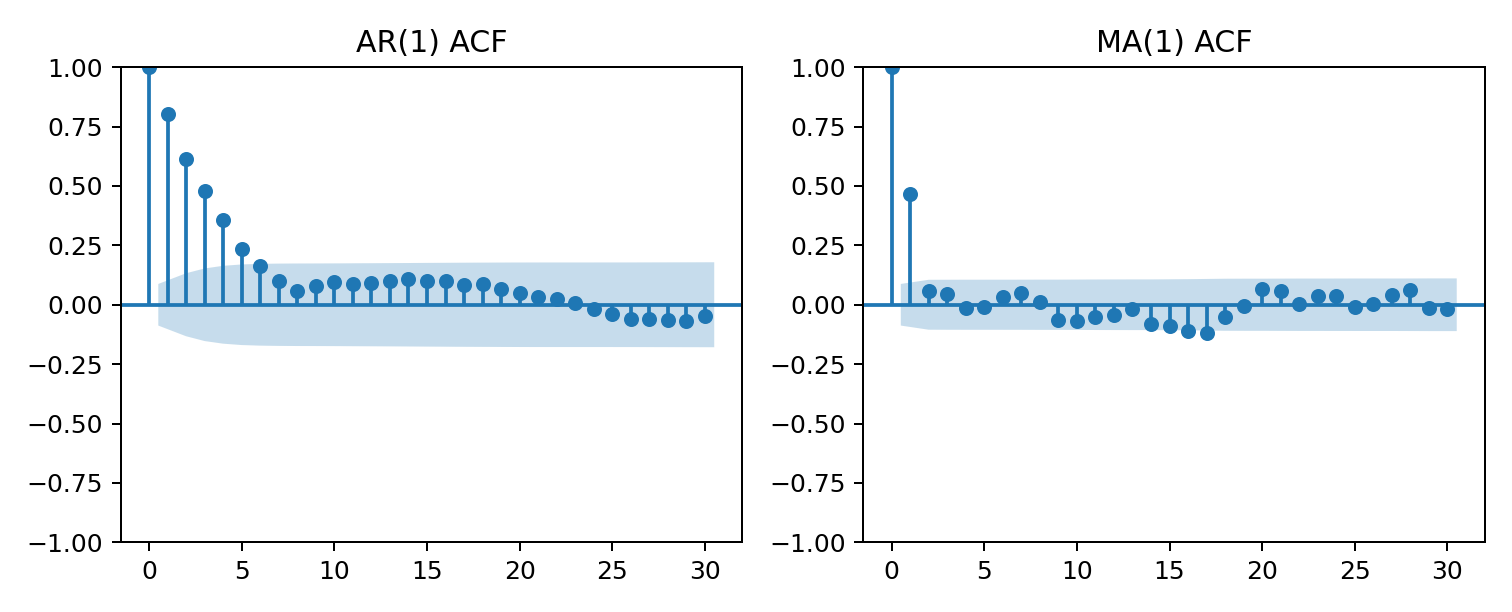
\includegraphics[width=0.86\textwidth]{ch06_fig01_acf_shapes.png}
  \caption{AR 与 MA 的 ACF 形态：AR 通常拖尾，MA 通常截尾。}
\end{figure}

\begin{figure}[htbp]
  \centering
  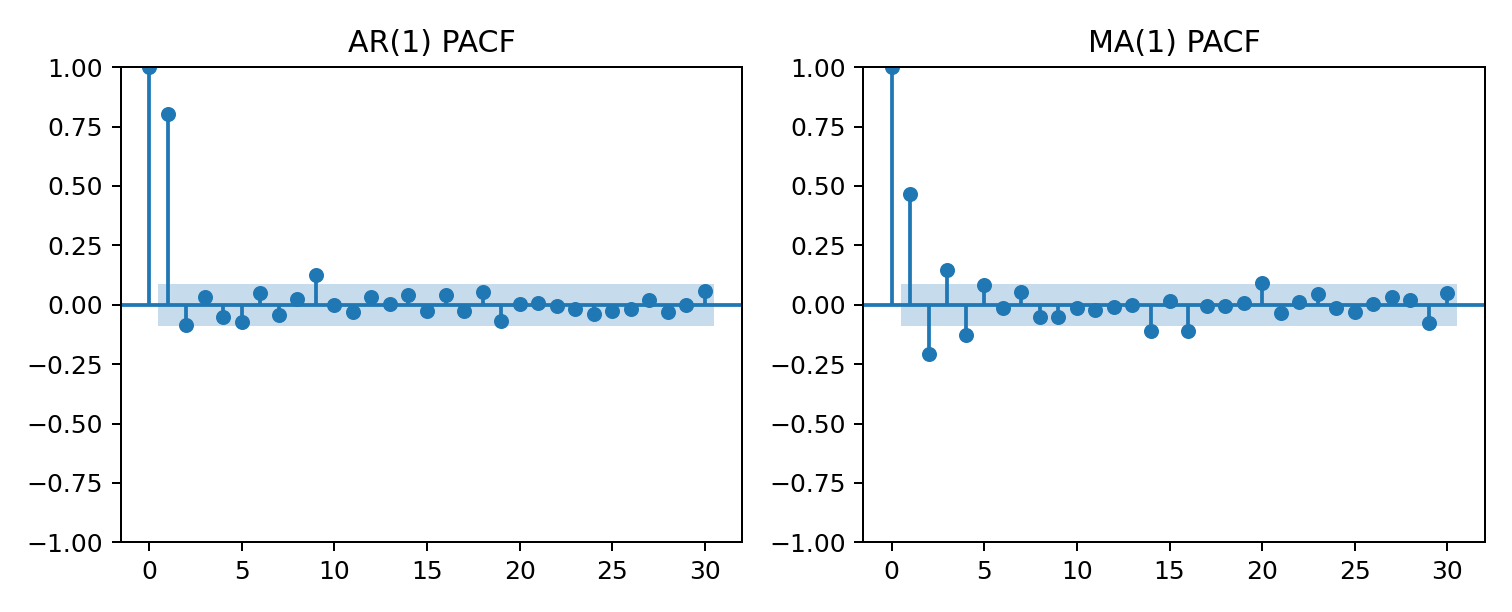
\includegraphics[width=0.86\textwidth]{ch06_fig02_pacf_shapes.png}
  \caption{AR 与 MA 的 PACF 形态：AR 通常截尾，MA 通常拖尾。}
\end{figure}

\section{练习提要}

原文练习主要围绕下列方向展开：
\begin{itemize}
  \item 推导 AR(2) 的自协方差和伪周期 ACF；
  \item 比较 AR、MA、ARMA 的 ACF/PACF 图；
  \item 计算 MA(1) 的偏相关；
  \item 证明 AR(p) 方差矩阵逆的带状结构。
\end{itemize}

\section*{本章小结}

第 6 章把线性模型与可观察的相关图联系起来。Yule-Walker 方程给出 AR 的协方差递推，MA 的协方差截尾，PACF 则将投影几何转化为模型识别工具。

\end{document}
